\chapter{Конструкторский раздел}
\label{cha:design}
\section{Общая архитектура приложения}
\begin{figure}[h!]
	\centering
	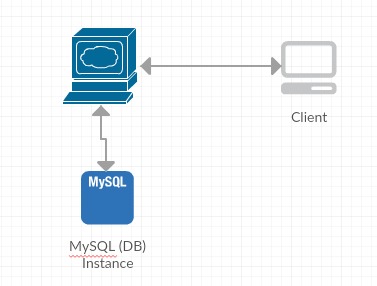
\includegraphics[width=0.4\textwidth]{img/img5.png}
	\caption{Общая архитектура приложения}
	\label{fig:spire09}
\end{figure}
Приложение построено по архитектуре "клиент-сервер". Клиент запускает на своём компьютере приложение и взаимодействует посредством сети с удаленным сервером. Сервер позволяет осуществлять доступ к необходимой информации из базы данных, разграничивать доступ пользователей к той или иной информации. Так же на сервере находится приложение, позволяющее парсить trace-файлы программы и заносить информацию в базу данных.
\section{PICL}
PICL (Portable Instrumented Communication Library)  - библиотека подпрограмм, разработанная в Oak Ridge National Laboratory (ORNL), которая реализует общий
нтерфейс передачи сообщений на множестве многопроцессорных архитектур. Программы, написанные с помощью примитивов PICL вместо команд среды взаимодействия, являются переносимыми в том смысле, что они могут выполняться на любой машине, для которой есть реализация PICL.\\
PICL была разработана для:
\begin{enumerate} 
\item Обеспечения переносимости между разными платформами с минимальными накладными расходами;
\item Получения трассировочных данных по межпроцессным взаимодействиям и пользовательским событиям, также с минимальными накладными расходами для избежания влияния на поведение исследуемой задачи, и
\item Обеспечения переносимости на новые системы, простого расширения для использования преимуществ новых команд конкретной системы
\end{enumerate} 
Для достижения этих целей PICL реализована как библиотека подпрограмм языка C с машинно-независимым трассировочным слоем и машинно-зависимым слоем, отображающимся на команды конкретной системы (когда это возможно). PICL  была открыта для широкого использования в марте 1989. Её разработка продолжалась, и были выпущены несколько релизов, добавляющие новые коммуникационные и трассировочные команды и поддержку новых вычислительных систем.
В последней версии PICL запись трассы имеет формат, показанный в таблице \ref{tab:tbl1}. Для каждой записи обязательными являются первые шесть полей, но если количество полей данных равно нулю, то дескриптор данных исключается.

\begin{table}[h!]
	\caption{\label{tab:tbl1}Формат записи трассы PICL}
\begin{tabular}{|l|l|}
	%	&\makebox[3em]{6/3}&\makebox[3em]{6/4}
	\hline
	Наименование поля & Назначение \\
	\hline\hline
	тип записи&тип информации в записи
	\\\hline
	тип события &тип события, с которым связана запись
	\\\hline
	отметка времени&когда информация была истинной\\\hline
	идентификатор процессора
	&процессор, с которым связана информация
	\\\hline
	идентификатор процесса	
	&процесс, с которым связана информация	
	\\\hline
	количество полей данных	
	&количество дополнительных полей данных, связанных \tabularnewline & с данными типами записи и события	
	\\\hline
	дескриптор данных	
	&формат полей данных
    \\\hline
    данные	
    &дополнительные поля данных
    \\\hline

\end{tabular}
\end{table}
Основное внимание в этом формате уделено записи информации, связанной как с системными, так и с пользовательскими событиями, при этом каждая запись связана с определённым типом события. Порядок полей записи отражает важность полей для систем, обрабатывающих данные: что, где, когда и ассоциированные с событием данные. Если тип записи или события не знаком системе, то данную запись можно пропустить. Но если система хочет получить информацию из записи, то ей для этого всё предоставлено.

Формат PICL предусматривает ранение данных в текстовом виде. Все поля состоят из символов кодировки ASCII и разделены пробелами. Тип записи, тип события, идентификаторы процессора и процесса, количество полей данных – целые числа. Дескриптор данных – это либо целое число, либо символьная строка переменной длины, заключённая в двойные кавычки. Формат полей данных определяется дескриптором данных. Временная метка – число с плавающей точкой, разрешение которой зависит от единиц измерения (например, секунд) и точности таймера на машине, на которой генерируется трасса.

    Практика показала, что текстовый формат очень полезен для переносимости, поиска и исправления ошибок в трассе и для возможной работы с трассой без помощи средств визуализации, и он не препятствует сжатию файлов, если это необходимо. При этом PICL использует двоичное представление данных при внутренней обработке для экономии места и избежания накладных расходов при преобразовании данных \cite{book4}.
Значения полей и их интерпретация приведены в таблице \ref{tab:tbl2}
\begin{table}[h!]
	\caption{\label{tab:tbl2} Значения полей записи}
	\begin{tabular}{|l|l|}
		%	&\makebox[3em]{6/3}&\makebox[3em]{6/4}
		\hline
		Поле & Назначение \\
		\hline\hline
		тип записи& $\geq0$ пользовательский тип записи\tabularnewline & $\le0$ стандартный системный тип записи
		\\\hline
		тип события & $\geq0$ пользовательское событие или определённое \tabularnewline & пользователем подмножество событий\tabularnewline & $=-1$ относится ко всем событиям \tabularnewline &(глобальная информация)
		\tabularnewline & $<-1$ системное событие или \tabularnewline &системное подмножество событий
		\\\hline
		временная метка& $\geq0$идентификатор конкретного процессора\tabularnewline & $=-1$ относится ко всем процессорам \tabularnewline &(глобальная информация)
		\tabularnewline & $<-1$ относится к подмножеству процессоров
		\\\hline
		идентификатор процесса
		&$\geq0$ идентификатор процесса\tabularnewline & на заданном процессоре\tabularnewline & $=-1$ относится ко всем процессам\tabularnewline & на заданном процессоре \tabularnewline &(глобальная информация)
		\tabularnewline & $<-1$ относится к подмножеству процессов\tabularnewline & на указанном процессоре
		\\\hline
		количество полей данных	
		&количество дополнительных полей данных	
		\\\hline
          дескриптор данных
		& если заключён в двойные кавычки,\tabularnewline & то формат функции scanf(),
		иначе:\tabularnewline &
		$=0$  символ ("\%c") \tabularnewline & $=1$ cтрока ("\%s") \tabularnewline &
		$=2$ целое число ("\%d") \tabularnewline &
		$=3$ длинное целое число  ("\%ld") \tabularnewline &
	    $=4$ число с плавающей точкой одинарной точности  ("\%f") \tabularnewline &
	    $=5$ число с плавающей точкой двойной точности   ("\%lf") \tabularnewline &
	    $>6$ другой предопределённый формат данных \tabularnewline &
	    
		
		\\\hline
	
	\end{tabular}
\end{table}
Идентификаторы процесса и процессора определяют «местоположение» события. Хотя обычно процессы на каждом процессоре нумеруются последовательно начиная с 0, может быть полезно нумеровать процессы независимо от процессора, прямо поддерживая как процессоро-зависимый, так и процессоро-независимый подход к визуализации. (Заметим, что на данный момент PICL не поддерживает много процессов на одном (последовательном) процессоре. Поле идентификатора процесса было введено для совместимости с системами, которые поддерживают эту модель и для возможности будущего расширения PICL. В трассах текущего формата идентификатору процесса присваивается либо действительной PID, т.е. номер процесса, заданный операционной системой, либо -1.)
\subsection{Технология обработки данных}
Формат трассы PICL, рассмотренный в предыдущем параграфе, предполагает единый формат записи как для событий профилируемой программы, так и для управляющих событий. Управляющие события описывают изменения формата трассы, которые должны быть учтены при её последующем разборе. Характерным примером такого события может служить описание нового формата данных.

Для программы, обрабатывающей эти данные более удобным было бы представление их в виде событий, характеризуемых временным интервалом, типом события и идентификатором процесса.
\section{Серверная часть}
Для хранения файлов трасс формата PICL была спроектирована база данных
\subsection{Базы данных}
\begin{lstlisting}[language=SQL]
CREATE TABLE Tracks ( 
filename VARCHAR(50) NOT NULL,
typeRecord INT NOT NULL,
typeEvent INT NOT NULL,
time FLOAT NOT NULL,
prid INT NOT NULL,
pid INT NOT NULL,
numData INT NOT NULL,
data VARCHAR(200),
FOREIGN KEY (typeEvent) REFERENCES Codes(code) 
ON DELETE CASCADE ON UPDATE CASCADE,
FOREIGN KEY (filename) REFERENCES Files(filename) 
ON DELETE CASCADE ON UPDATE CASCADE
) ENGINE = INNODB DEFAULT CHARSET=utf8;
\end{lstlisting}
Так же были спроектирована вспомогательные базы данных для хранения информации о событиях MPI, файлах, пользователях.
\begin{lstlisting}[language=SQL]
CREATE TABLE Users(
user  VARCHAR(50) NOT NULL  PRIMARY KEY,
password  VARCHAR(50) NOT NULL
) ENGINE = INNODB DEFAULT CHARSET=utf8;

CREATE TABLE Files(
filename  VARCHAR(50) NOT NULL PRIMARY KEY
) ENGINE = INNODB DEFAULT CHARSET=utf8;

CREATE TABLE FilesUsers(
user  VARCHAR(50) NOT NULL,
filename  VARCHAR(50) NOT NULL,
PRIMARY KEY (user, filename), 
FOREIGN KEY (filename) REFERENCES Files(filename)
ON DELETE CASCADE ON UPDATE CASCADE 
) ENGINE = INNODB DEFAULT CHARSET=utf8;

CREATE TABLE Codes(
code  INT NOT NULL  PRIMARY KEY,
name  VARCHAR(50) NOT NULL,
description TEXT,
category TEXT
) ENGINE = INNODB DEFAULT CHARSET=utf8;

\end{lstlisting} 

\subsection{API для взаимодействия с сервером}
Была разработано API взаимодействия между клиентом и сервером. Безопастность взаимодействия гарантируется тем, что взаимодействия осуществляется на основе токенов. Все запросы, кроме запроса на авторизацию, требуют содержания в себе уникального токена.Токен дается клиенту после успешного прохождения авторизации. То
\begin{lstlisting}[language=c++]
(*\bfseries [GET] /authenticate *)
Авторизация
Аргументы
)name - логин
)password - пароль

(*\bfseries [Example response]*)
{
"success": true,
"message": "Enjoy your token!",
"token": "eyJhbGciOiJIUzI1NiIsInR5cCI6IkpXVCJ9.eyJ1c2VyIj
oiVXNlciIsInBhc3N3b3JkIjoicHdkI
iwiaWF0IjoxNDk2NDM4ODc4LCJleHAiOjE0OT
Y1MjUyNzh9.0bhg6Ct8YXOGixVY-ZukmdVj
-35AE0BSZExGWJlpNKQ"
}

(*\bfseries[GET] /getFile*)
Получение куска содержанимого файла
Аргументы
)filename - имя файла
)offset - отступ от начала файла
)limit - количество получаемых записей
)timeMin - время начала записей
)timeMax - время конца записей

(*\bfseries [Example response]*)
{
"result": [
{
"filename": "trace1",
"typeRecord": -3,
"typeEvent": -901,
"time": 0.000007,
"prid": 0,
"pid": 0,
"numData": 0,
"data": "-1"
}],
}

(*\bfseries[GET] /getTimeBorders*)
Получение временного интервала трассы
Аргументы
)filename - имя файла

(*\bfseries [Example response]*)
{
"result": [
{
"MIN(time)": 0.000007000000096013537,
"MAX(time)": 0.11629900336265564
}],
}

(*\bfseries[GET] /getFileList*)
Получение списка файлов, доступных для данного пользователя
Аргументы
)name - логин

(*\bfseries [Example response]*)
{
"success": true,
"message": [
{
"filename": "trace1"
},
{
"filename": "trace2"
}],
}

(*\bfseries[GET] /getNumRecords*)
Получение количества записей для данного файла
Аргументы
)filename - имя файла
)timeMin - время начала записей
)timeMax - время конца записей
 
 (*\bfseries [Example response]*)
 {
 "result": [
 {
 "COUNT": 522
 }],
 }
 
(*\bfseries[GET] /getCodeInfo*)
Получение информации о событие по его коду
Аргументы
)code - код события

(*\bfseries [Example response]*)
{
"result": [
{
"name": "WILDCARD",
"description": "wildcard for all or any processes",
"category": "event type definitions"
}],
}

(*\bfseries[GET] /getNumProcess*)
Получение максимального количества процессов, которые записаны в файл
Аргументы
)filename - имя файла

(*\bfseries [Example response]*)
{
"result": [
{
"max(prid)": 7
}],
}
\end{lstlisting}

\section{Нормальные формы}
Нормальная форма — свойство отношения в реляционной модели данных, характеризующее его с точки зрения избыточности, потенциально приводящей к логически ошибочным результатам выборки или изменения данных. Нормальная форма определяется как совокупность требований, которым должно удовлетворять отношение.
Процесс преобразования отношений базы данных (БД) к виду, отвечающему нормальным формам, называется нормализацией. Нормализация предназначена для приведения структуры БД к виду, обеспечивающему минимальную логическую избыточность, и не имеет целью уменьшение или увеличение производительности работы или же уменьшение или увеличение физического объёма базы данных. Конечной целью нормализации является уменьшение потенциальной противоречивости хранимой в базе данных информации. Как отмечает К. Дейт, общее назначение процесса нормализации заключается в следующем:
\begin{enumerate}

	\item исключение некоторых типов избыточности;
	\item устранение некоторых аномалий обновления;
	\item разработка проекта базы данных, который является достаточно «качественным» представлением реального мира, интуитивно понятен и может служить хорошей основой для последующего расширения;
	\item упрощение процедуры применения необходимых ограничений целостности.

\end{enumerate}
Устранение избыточности производится, как правило, за счёт декомпозиции отношений таким образом, чтобы в каждом отношении хранились только первичные факты (то есть факты, не выводимые из других хранимых фактов)\cite{book6}.

\textbf{Первая нормальная форма}. Переменная отношения находится в первой нормальной форме тогда и только тогда, когда в любом допустимом значении отношения каждый его кортеж содержит только одно значение для каждого из атрибутов.
В реляционной модели отношение всегда находится в первой нормальной форме по определению понятия отношение.
Что же касается различных таблиц, то они могут не быть правильными представлениями отношений и, соответственно, могут не находиться в 1NF. В соответствии с определением К. Дж. Дейта для такого случая, таблица нормализована (эквивалентно — находится в первой нормальной форме) тогда и только тогда, когда она является прямым и верным представлением некоторого отношения. Конкретнее, рассматриваемая таблица должна удовлетворять следующим пяти условиям:
\begin{enumerate}
\item Нет упорядочивания строк сверху-вниз (другими словами, порядок строк не несет в себе никакой информации).
\item Нет упорядочивания столбцов слева-направо (другими словами, порядок столбцов не несет в себе никакой информации).
\item Нет повторяющихся строк.
\item Каждое пересечение строки и столбца содержит ровно одно значение из соответствующего домена.
\item Все столбцы являются обычными (в таблице нет «скрытых» компонентов, которые могут быть доступны только в вызове некоторого специального оператора взамен ссылок на имена регулярных столбцов).
\end{enumerate}
В моей базе данных каждый кортеж всех таблиц содержит только атомарные атрибуты (атрибут атомарен, если его значение теряет смысл при любом разбиении на части или переупорядочивании), отсутствуют повторяющиеся кортежи. Исходя из этого, можно сказать, что все таблицы находятся в первой нормальной форме.

\textbf{Вторая нормальная форма}. Переменная отношения находится во второй нормальной форме тогда и только тогда, когда она находится в первой нормальной форме и каждый неключевой атрибут неприводимо зависит от её потенциального ключа.
Неприводимость означает, что в составе потенциального ключа отсутствует меньшее подмножество атрибутов, от которого можно также вывести данную функциональную зависимость. Для неприводимой функциональной зависимости часто используется эквивалентное понятие «полная функциональная зависимость». Если потенциальный ключ является простым, то есть состоит из единственного атрибута, то любая функциональная зависимость от него является неприводимой (полной). Если потенциальный ключ является составным, то согласно определению второй нормальной формы в отношении не должно быть неключевых атрибутов, зависящих от части составного потенциального ключа.
Вторая нормальная форма по определению запрещает наличие неключевых атрибутов, которые вообще не зависят от потенциального ключа. Таким образом, вторая нормальная форма запрещает создавать отношения как несвязанные (хаотические, случайные) наборы атрибутов.
В моей базе данных не все потенциальные ключи состоят из одного атрибута, следовательно, нельзя сказать, что все таблицы находятся во второй нормальной форме.
\section{Архитектура клиентского приложения}
%%% Local Variables:

%%% mode: latex
%%% TeX-master: "rpz"
%%% End:
%--количество цветов
%||количество пикселей